\documentclass[10pt]{amsart}
\usepackage{times,amsmath,amsbsy,amssymb,amscd,mathrsfs}
\usepackage{slashbox}\usepackage{booktabs,graphicx,subfigure,epstopdf,wrapfig,chemarrow}

\usepackage{algorithm2e} 
\usepackage{multicol,multirow}
\usepackage{mathtools}
\usepackage[usenames,dvipsnames,svgnames,table]{xcolor}
\usepackage[all]{xy}
\usepackage{wrapfig}
\usepackage{tcolorbox}
\usepackage{stmaryrd}
%\usepackage[labelformat=simple]{subfig}
%\usepackage[hang,small,bf]{caption}

\usepackage{tikz,tikz-cd}
\usepackage[utf8]{inputenc}
\usepackage{pgfplots} 
\usepackage{pgfgantt}
\usepackage{pdflscape}
\pgfplotsset{compat=newest} 
\pgfplotsset{plot coordinates/math parser=false}
\newlength\fwidth

%\usepackage[notcite,notref]{showkeys}
\usepackage[numbered]{mcode}

\definecolor{myBlue}{rgb}{0.0,0.0,0.55}
%\definecolor{green}{rgb}{0.0,0.7,0.2}
\usepackage[pdftex,colorlinks=true,citecolor=myBlue,linkcolor=myBlue]{hyperref}

\usepackage[hyperpageref]{backref}
\usepackage{circledsteps}

%\newcommand{\LC}[1]{\textcolor{cyan}{#1}}
\newcommand{\LC}[1]{\textcolor{red}{#1}}

\usepackage{comment,enumerate,multicol,xspace}

  \newcounter{mnote}
  \setcounter{mnote}{0}
  \newcommand{\mnote}[1]{\addtocounter{mnote}{1}
    \ensuremath{{}^{\bullet\arabic{mnote}}}
    \marginpar{\footnotesize\em\color{red}\ensuremath{\bullet\arabic{mnote}}#1}}
  \let\oldmarginpar\marginpar
    \renewcommand\marginpar[1]{\-\oldmarginpar[\raggedleft\footnotesize #1]%
    {\raggedright\footnotesize #1}}

%\usepackage[pdftex,dvipsnames]{xcolor}

%\usepackage{xargs} % Use more than one optional parameter in a new commands
%\usepackage[colorinlistoftodos,prependcaption,textsize=footnotesize]{todonotes}
%
%\newcounter{mycomment}
%\newcommand{\mycomment}[2][]{%
%% initials of the author (optional) + note in the margin
%\refstepcounter{mycomment}%
%{%
%\todo[linecolor=blue,backgroundcolor=blue!25,bordercolor=blue]{%
%\textbf{Comment [{\sc #1\themycomment}]:}\\#2}%
%}}
%
%\newcommandx{\change}[2][1=]
%{\todo[linecolor=OliveGreen,backgroundcolor=OliveGreen!25,bordercolor=OliveGreen,#1]{%
%{\sc Change}:\\#2}}
%
%\newcommandx{\improvement}[2][1=]
%{\todo[linecolor=Plum,backgroundcolor=Plum!25,bordercolor=Plum,#1]{%
%{\sc Improvement}:\\#2}}
%
%\newcommandx{\unsure}[2][1=]
%{\todo[linecolor=red,backgroundcolor=red!25,bordercolor=red,#1]{%
%{\sc Unsure}:\\ #2}}
%

% \newcommand{\mnote}[1]{}
\newcommand{\breakline}{
\begin{center}
------------------------------------------------------------------------------------------------------------
\end{center}
}
%\usepackage{geometry}
%%\usepackage{graphicx,pst-eps,epstopdf}
%\geometry{letterpaper, margin=1.5in}

\newtheorem{theorem}{Theorem}[section]
\newtheorem{lemma}[theorem]{Lemma}
\newtheorem{corollary}[theorem]{Corollary}
\newtheorem{proposition}[theorem]{Proposition}
\newtheorem{definition}[theorem]{Definition}
\newtheorem{example}[theorem]{Example}
\newtheorem{exercise}[theorem]{Exercise}
\newtheorem{question}[theorem]{Question}
\newtheorem{remark}[theorem]{Remark}
\newtheorem{alg}[theorem]{Algorithm}
%\newtheorem{answer}[proof]{Question}

\newcommand{\dx}{\,{\rm d}x}
\newcommand{\dd}{\,{\rm d}}
\newcommand{\deq}{\stackrel{\rm def}{=}}
\newcommand{\mbb}{\mathbb}
\newcommand{\mbf}{\bs}
\newcommand{\bs}{\boldsymbol}
\newcommand{\mcal}{\mathcal}
\newcommand{\mc}{\mcode}
\newcommand{\lla}{\langle}
\newcommand{\rra}{\rangle}
\newcommand{\supp}{\operatorname{supp}}
\newcommand{\range}{\operatorname{range}}
\newcommand{\PartSize}{\fontsize{0.85cm}{0.85cm}\selectfont} 
\newcommand{\mscr}{\mathscr}
\DeclarePairedDelimiter\ceil{\lceil}{\rceil}
\DeclarePairedDelimiter\floor{\lfloor}{\rfloor}

%\newcommand{\span}{\rm span}
\newcommand{\red}{\color{red}}
\newcommand{\green}{\color{green}}
\newcommand{\blue}{\color{blue}}
\newcommand{\gray}{\color{gray}}

%\DeclareMathOperator*{\curl}{curl}
\DeclareMathOperator*{\img}{img}
%\DeclareMathOperator*{\span}{span}
\DeclareMathOperator*{\diag}{diag}
\newcommand{\curl}{{\rm curl\,}}
\renewcommand{\div}{\operatorname{div}}
%\renewcommand{\grad}{\operatorname{grad}}
\newcommand{\grad}{{\rm grad\,}}
\DeclareMathOperator*{\tr}{tr}
\DeclareMathOperator*{\rot}{rot}
\DeclareMathOperator*{\var}{Var}
\DeclareMathOperator{\rank}{rank}

\newcommand{\step}[1]{\noindent\raisebox{1.5pt}[10pt][0pt]{\tiny\framebox{$#1$}}\xspace}

%\usepackage[margins]{trackchanges}
%\renewcommand{\initialsOne}{chen}

\newcommand{\dual}[1]{\left\langle {#1} \right\rangle}
\newcommand{\norm}[1]{\left\Vert#1\right\Vert}
\newcommand{\snorm}[1]{\left\vert#1\right\vert}
\newcommand{\vertiii}[1]{{\left\vert\kern-0.25ex\left\vert\kern-0.25ex\left\vert #1 
    \right\vert\kern-0.25ex\right\vert\kern-0.25ex\right\vert}}


\begin{document}
\title{ODE Solvers: One-Step Methods}
\author{Long Chen}\date{\today}
\begin{abstract}
This is my brief summary of Chapter 5 and 6 of the book {\em Numerical Analysis} by {\em Gautschi, Walter}. Discussion is simplified and more figures are provided for a better illustration. 
\end{abstract}
\maketitle

\tableofcontents

We consider numerical methods for solving the nonlinear ODE  
\begin{equation}\label{ODE}  
y' = f(t,y),\quad y(a) = y_0,  
\end{equation}  
where $t \in \mathbb{R}$ is the independent variable, $y = y(t) \in \mathbb{R}^d$ may be a vector-valued function, and the function $f(t, y)$ is given. Assume $f(t, y)$ is Lipschitz continuous with respect to $y$, i.e., $\|f(t, y_1) - f(t, y_2)\| \leq L\|y_1 - y_2\|$. Under this condition, the solution $y$ to \eqref{ODE} exists and is unique, at least in a neighborhood of $a$. We further assume that the solution exists for all $t \in \mathbb{R}$. The focus here is on how to compute a numerical approximation of $y$.  

A noticeable difference from the textbook {\em Numerical Analysis} by {\em Gautschi, Walter} is that the independent variable is changed from $x$ to $t$, which more naturally represents time.  


\section{Schemes}
\subsection{Forward Euler Method}  
Besides the initial value $y_0$, equation \eqref{ODE} also provides the initial derivative $y'(a) = f(a, y_0)$. Using the Taylor expansion, we obtain  
$$y(a+h) \approx y(a) + h y'(a) = y_0 + h f(a, y_0).$$  
To clearly distinguish between the exact solution $y$ to \eqref{ODE} and its numerical approximation, we introduce the notation $u_n$ for the numerical approximation, where the subscript $n$ corresponds to the grid point $t_n$. The step size, which may vary at each iteration, is denoted by $h_n$.  

The simplest forward (explicit) Euler method can be summarized as follows:  

\medskip  
\begin{tcolorbox}[colframe=black!15!white, coltitle=white!5!black, title = \bf Forward/Explicit Euler Method]  
Let $t_0 = a$, $u_0 = y_0$. For $n = 0, 1, 2, \dots$,  
\begin{align*}  
t_{n+1} &= t_n + h_n, \\  
u_{n+1} &= u_n + h_n f(t_n, u_n).  
\end{align*}  
\end{tcolorbox}  

Geometrically, the exact solution $y$ to \eqref{ODE} is a curve, and the Euler method approximates this curve using a polygon; see Fig. \ref{fig:ODEsolver}. Intuitively, as the length of each side of the polygon approaches zero, the numerical approximation can closely approximate the true solution. Numerical analysis provides a mathematical framework to rigorously analyze the error and, when possible, improve the methods.  

\begin{figure}[htbp]
\begin{center}
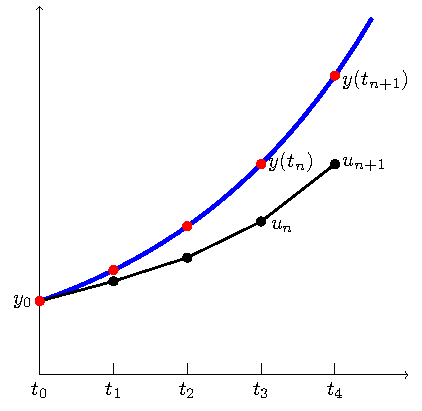
\includegraphics[width=7cm]{figures/ODEsolver.pdf}
\caption{An example of one step method.}
\label{fig:ODEsolver}
\end{center}
\end{figure}

\medskip
\noindent {\bf Question}: Euler method can be understood as moving along the tangential direction with a small step size. Is there any better direction to move? 
\medskip

\subsection{One step method and truncation error}
We first provide a measure of how ``good" a method is. Consider a single interval $[t_n, t_{n+1}]$. The step size $h_n := t_{n+1} - t_n$ may vary but is usually uniform. A generic form of a one-step method is given by  
\begin{equation}\label{onestep}  
u_{n+1} = u_n + h_n \Phi(t_n, u_n; h_n),  
\end{equation}  
where $\Phi(t_n, u_n; h_n)$ represents the direction of movement starting from $(t_n, u_n)$. For the forward Euler method, $\Phi(t_n, u_n; h_n) = f(t_n, u_n)$.  

Now consider the ODE \eqref{ODE}, $y' = f(t, y)$, restricted to the interval $[t_n, t_{n+1}]$ with the initial condition $y(t_n) = y_n$. The exact solution value at $t_{n+1}$ is denoted by $y_{n+1} = y(t_{n+1})$.  

Assume $u_n = y_n$ and use the error $u_{n+1} - y_{n+1}$ as a measure of accuracy. It is easy to see that this error is proportional to the step size. To provide a more consistent comparison, we define the normalized quantity  
$$T(t_n, y_n; h_n) := \frac{1}{h_n}(u_{n+1} - y_{n+1}),$$  
which is referred to as the {\em truncation error}.  

For simplicity, we omit the subscript $n$ and use the subscript $_{\rm next}$ to indicate $n+1$. With this notation, the truncation error can be rewritten as  
$$T(t, y; h) = \frac{1}{h}(u_{\rm next} - y_{\rm next}).$$  

This relationship is summarized in the following figure.  

\begin{figure}[htbp]
\begin{center}
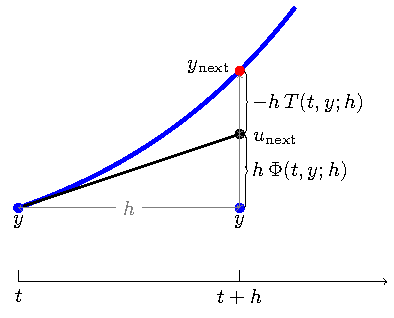
\includegraphics[width=7.5cm]{figures/TruncationError.pdf}
\caption{One step method and its truncation error.}
\label{fig:Th}
\end{center}
\end{figure}

Note that we add a negative sign in front of the truncation error in Fig. \ref{fig:Th}. The reason is that the length of a line segment is always positive, but by the definition of $T$, it can take negative values. For the example in the figure, $T$ is negative, and $-hT$ represents the distance.  

\begin{definition}[Order of a method]
The method is said to have order $p$ if, for some vector norm $\|\cdot\|$,  
\begin{equation}\label{eq:order_p}
\|T(t, y; h)\| \leq C h^p,  
\end{equation}  
uniformly on $[a, b] \subset \mathbb{R}^d$, with a constant $C$ not depending on $t$, $y$, or $h$.  
We express this property briefly as  
\begin{equation}\label{eq:order_bigO}
T(t, y; h) = \mathcal{O}(h^p), \quad h \to 0.  
\end{equation}  

Note that $p > 0$ implies consistency. Usually, $p$ is an integer $\geq 1$. It is called the \emph{exact order} if \eqref{eq:order_p} does not hold for any larger $p$.  
\end{definition}

\begin{definition}[Principal error function]
A function $\Psi: [a, b] \subset \mathbb{R}^d \to \mathbb{R}^d$ that satisfies $\Psi(t, y) \neq 0$ and  
\begin{equation}\label{eq:principal_error}
T(t, y; h) = \Psi(t, y) h^p + \mathcal{O}(h^{p+1}), \quad h \to 0,  
\end{equation}  
is called the \emph{principal error function}.
\end{definition}

Using the definition of the one-step method (cf. \eqref{onestep}) and the fact that $y' = f(t, y)$, the truncation error can also be expressed as  
\begin{equation}\label{eq:Tphi}  
T(t, y; h) = \Phi(t, y; h) - \frac{1}{h} \int_{t}^{t+h} f(s, y(s)) \, \dd s.  
\end{equation}  
This shows that the truncation error represents the discrepancy between the numerical quadrature $\Phi(t, y; h)$ and the average of $f(t, y(t))$ over the interval $[t, t+h]$.  

From this perspective, we can immediately see that the forward Euler method has a first-order truncation error:  
$$  
T_{\rm Euler}(t, y; h) = f(t, y(t)) - \frac{1}{h} \int_{t}^{t+h} f(s, y(s)) \, \dd s = \mathcal{O}(h).  
$$  
If we use the midpoint rule or the trapezoidal rule for the integral, the order of accuracy improves to second order. In general, numerical quadrature rules of arbitrary order can be applied.  

%However, what additional challenges arise when using such methods to solve ODEs?  
For instance, by performing a Taylor expansion at $t + h/2$, we find:  
$$  
f\left(t + \frac{h}{2}, y\left(t + \frac{h}{2}\right)\right) - \frac{1}{h} \int_{t}^{t+h} f(s, y(s)) \, \dd s = \mathcal{O}(h^2).  
$$  
What is the extra difficulty here compared to standard numerical quadrature?  

\subsection{Second-order methods}
The difference and difficulty lie in the fact that $y(t + \frac{h}{2})$ is unknown; we only have the initial value $y(t)$. How can we address this? One approach is to use the forward Euler method to advance by $h/2$ and obtain $u_{\rm half}$ as an approximation of $y(t + \frac{h}{2})$. Specifically, we approximate $f(t + \frac{h}{2}, y(t + \frac{h}{2}))$ with $f(t + \frac{h}{2}, u_{\rm half})$. This leads to the update formula:  
$$  
u_{\rm next} = u + h f\left(t + \frac{h}{2}, u + \frac{h}{2} f(t, u)\right).  
$$  

In practice, we can unfold the nested expressions of $f$ to derive the following improved Euler method:  

\medskip  
\begin{tcolorbox}[colframe=black!15!white, coltitle=white!5!black, title = \bf Improved Euler Method]  
Let $t_0 = a$, $u_0 = y_0$. For $n = 0, 1, 2, \dots$,  
\begin{align*}  
k_1 &= f(t_n, u_n), \\  
k_2 &= f(t_n + h_n/2, u_n + k_1 h_n/2), \\  
u_{n+1} &= u_n + h_n k_2.  
\end{align*}  
\end{tcolorbox}  

The direction $k_2$ is an improvement over $k_1$ because it reduces the truncation error to $\mathcal{O}(h^2)$.  

Similarly, by modifying the trapezoidal method for numerical quadrature, we obtain a method known as the Heun method. It is also a second-order method.  

\medskip
\begin{tcolorbox}[colframe=black!15!white, coltitle=white!5!black, title = \bf Heun Method]
Let $t_0=a,\, u_0 = y_0$. For $n=0,1,2,...,$
\begin{align*}
k_1 &= f(t_n, u_n),\\
k_2 & = f(x_n + h_n, u_n + k_1h_n),\\
u_{n+1} &= u_n + h_n (k_1 + k_2)/2.
\end{align*}
\end{tcolorbox}

\begin{figure}[htbp]
\begin{center}
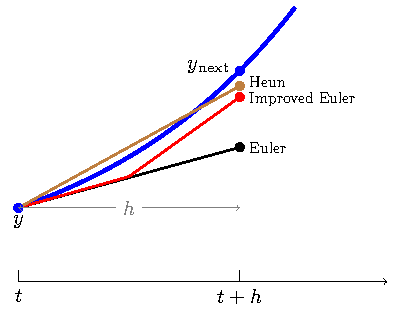
\includegraphics[width=7.25cm]{figures/EulerMethod.pdf}
\caption{Forward Euler, improved Euler and Heun methods}
\label{fig:EulerMethod}
\end{center}
\end{figure}


Notice that both the modified Euler method and Heun's method require evaluating the slope twice; see Fig.~\ref{fig:EulerMethod}. These are special cases of two-stage methods, which will be discussed below.  

\subsection{Two-stage methods}  

A generic form of two-stage methods is given by  
\begin{equation}\label{eq:twostage}  
u_{\rm next} = u + (\alpha_1 h) k_1 + (\alpha_2 h) k_2,  
\end{equation}  
where the weight $\alpha_1 \in [0,1)$, and $\alpha_1 + \alpha_2 = 1$. The geometric interpretation is that we first move along the direction $k_1$ with a step size of $\alpha_1 h$ and then switch to a better direction $k_2$ for the remaining step size.  

We introduce another parameter $\mu \in (0,1]$ and treat $k_2$ as an approximation of the slope at $(t + \mu h, y(t + \mu h))$. Since $y(t + \mu h)$ is unknown, it is approximated using the forward Euler method, i.e., $k_2 = f(t + \mu h, y + \mu h k_1)$.  

Next, we aim to choose the parameters $(\alpha_1, \alpha_2, \mu)$ to minimize the truncation error as formulated in \eqref{eq:Tphi}. The primary tool for this is a Taylor expansion at the left endpoint $(t, y)$. First,  
\begin{align*}  
k_2 &= f(t + \mu h, y + \mu h k_1) \\  
&= f + \mu h f_t + \mu h k_1 f_y + \frac{1}{2} \left[ \mu^2 h^2 f_{tt} + 2 \mu^2 h^2 f_{ty} k_1 + \mu^2 h^2 k_1^{\intercal} f_{yy} k_1 \right] + \mathcal{O}(h^3).  
\end{align*}  
Recall that $k_1 = f = f(t, y)$. Substituting this into the expression for $\Phi(t, y; h)$, we obtain  
\begin{align*}  
\Phi(t, y; h) &= \alpha_1 k_1 + \alpha_2 k_2 \\  
&= f + \alpha_2 \mu h (f_t + f_y f) + \frac{\alpha_2}{2} \mu^2 h^2 \left[ f_{tt} + 2 f_{ty} f + f^{\intercal} f_{yy} f \right] + \mathcal{O}(h^3).  
\end{align*}  

Then we compare $\Phi(t, y; h)$ with $\frac{1}{h} \int_{t}^{t+h} f(s, y(s)) \, \dd s$. We expand the integrand \( f(s, y(s)) \) at \((t, y)\):  
\begin{equation}\label{eq:fTaylor}  
f(s, y(s)) = f + \frac{\dd f}{\dd s}(s - t) + \frac{1}{2} \frac{\dd^2 f}{\dd s^2}(s - t)^2 + \mathcal{O}(h^3).  
\end{equation}  
Since the second variable \( y \) is also a function of the first one, the derivatives, by the chain rule, are given as  
\begin{align*}  
f^{[1]}(t, y(t)) &:= \frac{\dd f}{\dd t}(t, y(t)) = f_t + f_y y' = f_t + f_y f, \\  
f^{[2]}(t, y(t)) &:= \frac{\dd f^{[1]}}{\dd t}(t, y(t)) = f_t^{[1]} + f_y^{[1]} f \\  
&= f_{tt} + 2 f_{ty} f + f^{\intercal} f_{yy} f + f_y f^{[1]}.  
\end{align*}  
Higher derivatives \( f^{[k]} := \frac{\dd^k f}{\dd t^k} \) can be computed recursively.  

Substituting \eqref{eq:fTaylor} into \( h^{-1} \int_{t}^{t+h} f(s, y(s)) \dd s \), and combining this with the expansion of \( \Phi \), we obtain  
\begin{align*}  
T(t, y; h) = & (\alpha_1 + \alpha_2 - 1) f + \left( \alpha_2 \mu - \frac{1}{2} \right) h f^{[1]} - \red{\frac{1}{6} h^2 f_y f^{[1]}} \\  
& + \frac{1}{2} h^2 \left( \alpha_2 \mu^2 - \frac{1}{3} \right) (f_{tt} + 2 f_{ty} f + f^{\intercal} f_{yy} f) + \mathcal{O}(h^3).  
\end{align*}  

Since the \textcolor{red}{red term} is generally nonzero, the two-stage methods are limited to at most second-order accuracy. We achieve second-order accuracy by choosing parameters that satisfy the relations  
\[
\alpha_1 + \alpha_2 = 1, \quad \alpha_2 \mu = \frac{1}{2}.
\]  

Examples of $(1- \alpha_2, \alpha_2, 1/(2\alpha_2))$ include
\begin{itemize}
 \item Improved Euler method: $(0, 1, 1/2)$;
 \item Heun method: $(1/2, 1/2, 1)$;
 \item The choice $(1/4, 3/4, 2/3)$ will remove one part in $h^2$ term.
\end{itemize}
Notice that the choice \((1, 0, 0)\) corresponds to the forward Euler method, which only achieves a truncation order of \( \mathcal{O}(h) \).  


\subsection{Runge-Kutta methods}
A generalization of two-stage methods is $r$-stage Runge-Kutta methods:
\begin{align*}
\Phi(t, y; h) &= \sum_{s=1}^r \alpha_s k_s,\\
k_1 &= f(t, y);\\
k_s & = f(t+\mu_s h, y + h \sum_{j=1}^{s-1}\lambda_{sj}k_j), \quad s = 2,3,\ldots, r.
\end{align*}
The maximal order of $r$-stage R-K method is bounded by $r$ and only achievable for $r\leq 4$. Systematical way of finding parameters can be found in ... Here we only list a popular one.

\begin{figure}[htbp]
\begin{center}
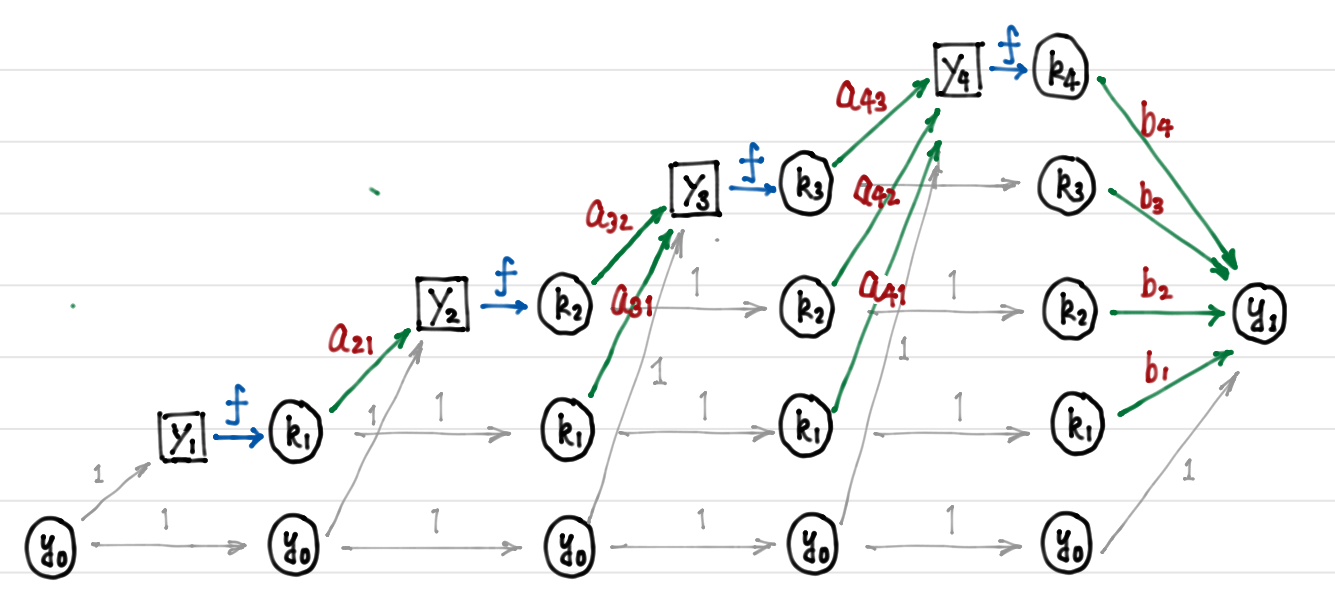
\includegraphics[width=3.6in]{figures/RK.png}
\caption{Runge-Kutta method}
\label{fig:RK}
\end{center}
\end{figure}

\begin{tcolorbox}[colframe=black!15!white, coltitle=white!5!black, title = \bf The classical $4$-th order Runge-Kutta method]
Let $t_0=a,\, u_0 = y_0$. For $n=0,1,2,...,$
\begin{align*}
k_1 &= f(t_n, u_n),\\
k_2 & = f(t_n + \frac{1}{2}h_n, u_n + \frac{1}{2}h_n k_1),\\
k_3 & = f(t_n + \frac{1}{2}h_n, u_n + \frac{1}{2}h_n k_2),\\
k_4 & = f(t_n + h_n, u_n + h_n k_3),\\
u_{n+1} &= u_n +  \frac{h_n}{6}( k_1 + 2k_2 + 2k_3 + k_4).
\end{align*}
\end{tcolorbox}

\section{Convergence Analysis}

\end{document}
\newpage

\section{Multi-Steps Methods}
We can use more information on the previous steps to get a higher order methods. It will be useful to introduce the following symbols representing indices, function value and derivative at various locations.

\begin{figure}[htbp]
\begin{center}
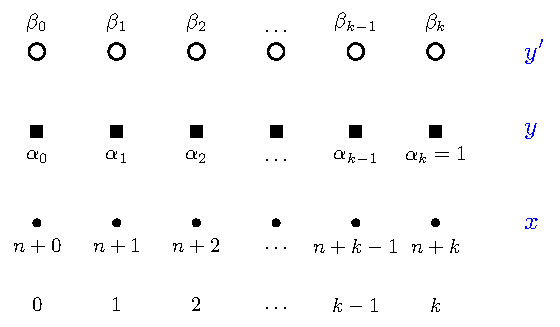
\includegraphics[width=9cm]{figures/multistep.pdf}
\caption{Notation for multi-step methods}
\label{fig:multistep}
\end{center}
\end{figure}

We use subscript to indicates the function evaluated at the corresponding grid points. For example, for $i=0,1,\ldots, k$
$$
y_{n+i} = y(x_{n+i}), \quad f_{n+i} = f(x_{n+i}, y(x_{n+i})).
$$
Depending on the context, sometimes $f_{n+i}$ could represent $f(x_{n+i}, u_{n+i})$.

\subsection{Adams-Bashforth method}
Recall that 
\begin{equation}
y_{n+k} = y_{n+k-1} + \int_{x_{n+k-1}}^{x_{n+k}} y'(t)\dd t = y_{n+k-1} + \int_{x_{n+k-1}}^{x_{n+k}} f(x, y(x))\dx.
\end{equation}

Suppose we know function values $y_{n+i}$ for $i=0,\ldots, k-1$, we can evaluate to get $f_{n+i}$ and fit the data $(x_{n+i}, f_{n+i})$ with a polynomial of degree $k-1$. For example, the Lagrange interpolant $f_I$ to $f$ can be written as 
$$
f_I(x) = \sum_{i=0}^{k-1}p_i(x) f_{n+i},
$$
where $p_i(x)\in \mathbb P_{k-1}$ and $p_i(x_{n+j}) = \delta_{ij}$. 

\begin{figure}[htbp]
\begin{center}
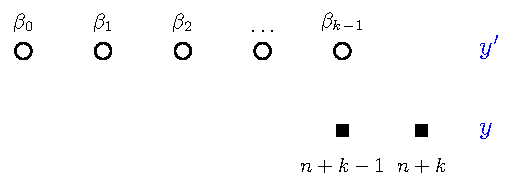
\includegraphics[width=8cm]{figures/ABmethod.pdf}
\caption{Adams-Bashforth method}
\label{fig:multistep}
\end{center}
\end{figure}

Approximate $f$ by $f_I$ and let $$\beta_i = \frac{1}{h}\int_{x_{n+k-1}}^{x_{n+k}} p_i(x) \dx,$$ we then obtain the Adams-Bashforth method
\begin{equation}
u_{n+k} = u_{n+k-1} + h \sum_{i=0}^{k-1}\beta_i f_{n+i}.
\end{equation}

When studying the truncation error, we assume the function value $y_{n+i}$ is known for $i=0,1,\ldots,k-1$. Then the truncation error $$T_h^{\rm AB} := \frac{1}{h} (u_{n+k} - y_{n+k}) = \frac{1}{h} \int_{x_{n+k-1}}^{x_{n+k}} (f_I - f) \dx = \frac{1}{h} \int_{x_{n+k-1}}^{x_{n+k}} ((y')_I - y') \dx.$$
We switch the integrand to $y'$ since now the remainder can be written as derivative of exact solution $y$. As the Lagrange interpolant preserves polynomial  

\subsection{Adams-Moulton method}
The only difference is the point $(x_{n+k}, f_{n+k})$ is included to fit the polynomial. 
\begin{figure}[htbp]
\begin{center}
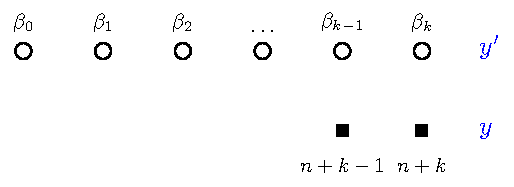
\includegraphics[width=8cm]{figures/AMmethod.pdf}
\caption{Adams-Moulton method}
\label{fig:multistep}
\end{center}
\end{figure}

Now the Lagrange interpolant $f_I$ to $f$ will be 
$$
f_I(x) = \sum_{i=0}^{k}p_i^*(x) f_{n+i},
$$
where $p_i^*(x)\in \mathbb P_{k}$ and $p_i^*(x_{n+j}) = \delta_{ij}$ for $i,j=0,1,\ldots, k$. The superscript $^*$ is introduced to distinguish the same quantity used in A-B method.

Approximate $f$ by $f_I$ and let $$\beta_i^* = \frac{1}{h}\int_{x_{n+k-1}}^{x_{n+k}} p_i^*(x) \dx,$$ we then obtain the Adams-Moultion method
\begin{equation}\label{AM}
u_{n+k} = u_{n+k-1} + h \sum_{i=0}^{k-1}\beta_i^* f_{n+i} + h\beta_k^*f(x_{n+k,} u_{n+k}).
\end{equation}
Here we single out the last term to emphasize A-M method is an implicit method and an iteration is needed to solve the nonlinear equation \eqref{AM}. 


\bibliographystyle{abbrv}
 \bibliography{/Dropbox/Math/biblib/library}
\end{document}